\documentclass[10pt]{beamer}

%STANDARD PREAMBLE
%https://tex.stackexchange.com/questions/68821/is-it-possible-to-create-a-latex-preamble-header
\usepackage{/Users/mwojno01/Repos/latex_preamble/beamer_preamble}

%
%% ALLOW FOR ITEMIZE ENVIRONMENTS WITH NO PRECEDING
% SPACING, IF DESIRED
% Reference: https://tex.stackexchange.com/questions/86054/how-to-remove-the-whitespace-before-itemize-enumerate
%\usepackage{enumitem}% http://ctan.org/pkg/enumitem 
\usepackage{paralist}


\title{Filtrations and Martingales}

\begin{document}

\maketitle


\begin{frame}{Review: $\sigma$-field}

Martingales depend on filtrations, which depend on $\sigma$-fields.

\begin{definition}
Let $\F$ be a collection of subsets of a set $\Omega$.  Then $\F$ is called a \textbf{sigma-field}  if it satisfies
%
\begin{enumerate}
	\item $\Omega \in \F$ 
	\item If $A \in \F$, then $A^c \in \F$.
	\item If $A_1,A_2, ... \in \F$ then $\cup_{i=1}^\infty A_i \in \F$.  
\end{enumerate}
%
that is, if $\Omega \in \F$ and $\F$ is closed under complementation and countable unions.
\label{def:sigma_field}	
\end{definition}


\begin{example}
Let $\Omega$ be the unit square, and  
\[ \F = \Bigg\{ 
 \begin{tikzpicture}[baseline=+2.0ex, scale=0.2]
   \draw         (0,0) rectangle  ++ (4,4);
 \end{tikzpicture},  \quad 
 
\begin{tikzpicture}[baseline=+2.0ex, scale=0.2]
   \draw         (0,0) rectangle  ++ (4,4);
  \fill[blue]    (0,0) rectangle  ++ (2,4);
 \end{tikzpicture},  \quad 
 
\begin{tikzpicture}[baseline=+2.0ex, scale=0.2]
  \draw         (0,0) rectangle  ++ (4,4);
  \fill[blue]    (2,0) rectangle  ++ (2,4);
  \end{tikzpicture}, \quad
 
\begin{tikzpicture}[baseline=+2.0ex, scale=0.2]
  \draw         (0,0) rectangle  ++ (4,4);
  \fill[blue]    (0,0) rectangle  ++ (4,4);
  \end{tikzpicture} 
 \Bigg\} \] 
\end{example} 

\end{frame}



\begin{frame}{Filtrations}
\begin{definition}
Let $(\Omega, \F, P)$ be a probability space. 

Then a \textbf{filtration} $\F_1 \subset \F_2 \subset \cdots$ is an increasing sequence of sub $\sigma$-fields of $\F$. 
	
\end{definition}	
\end{frame}

\begin{frame}{A simple strategy for constructing a filtration}

A simple method for constructing a filtration is as follows. 
%
\begin{enumerate}
	\item Construct a sequence $\set{\Omega_n}$ of increasingly refined partitions of $\Omega$.
	\item Define a filtration by setting $\F_n = \sigma(\Omega_n)$, i.e. each $\sigma$-field $\F_n$ consists of the sets that can be formed by taking unions of some subset of the cells in the partition $\Omega_n$.
\end{enumerate}
%
Some examples of filtrations formed by this strategy include:
%
\begin{enumerate}
	\item Take $\Omega$ to be the unit square. Form increasingly refined partitions by splitting cells of $\Omega_{n-1}$ in half, vertically if $n$ odd and horizontally if $n$ even.  
	\item  Let $\Omega$ be the space of binary-valued sequences. Form increasingly refined partitions by having $\Omega_{n}$ group together all sequences whose values match along the first $n$ coordinates. 
\end{enumerate}
\end{frame}


\begin{frame}{Example of a filtration}
Let $\Omega$ be the unit square.   Define $\set{\F_n}$ by

\begin{align*} 
 \F_0 &= \Bigg\{ 
 \begin{tikzpicture}[baseline=+2.0ex, scale=0.2]
   \draw         (0,0) rectangle  ++ (4,4);
 \end{tikzpicture},  \quad 
 
\begin{tikzpicture}[baseline=+2.0ex, scale=0.2]
  \draw         (0,0) rectangle  ++ (4,4);
  \fill[green]    (0,0) rectangle  ++ (4,4);
  \end{tikzpicture} 
 \Bigg\}  \\
 \F_1 &= \Bigg\{ 
 \begin{tikzpicture}[baseline=+2.0ex, scale=0.2]
   \draw         (0,0) rectangle  ++ (4,4);
 \end{tikzpicture},  \quad 
 
\begin{tikzpicture}[baseline=+2.0ex, scale=0.2]
   \draw         (0,0) rectangle  ++ (4,4);
  \fill[blue]    (0,0) rectangle  ++ (2,4);
 \end{tikzpicture},  \quad 
 
\begin{tikzpicture}[baseline=+2.0ex, scale=0.2]
  \draw         (0,0) rectangle  ++ (4,4);
  \fill[blue]    (2,0) rectangle  ++ (2,4);
  \end{tikzpicture}, \quad
 
\begin{tikzpicture}[baseline=+2.0ex, scale=0.2]
  \draw         (0,0) rectangle  ++ (4,4);
  \fill[blue]    (0,0) rectangle  ++ (4,4);
  \end{tikzpicture} 
 \Bigg\}  \\
  \F_2 &= \Bigg\{ 
 \begin{tikzpicture}[baseline=+2.0ex, scale=0.2]
   \draw         (0,0) rectangle  (4,4);
 \end{tikzpicture},  \quad 
 
\begin{tikzpicture}[baseline=+2.0ex, scale=0.2]
   \draw         (0,0) rectangle  (4,4);
  \fill[red]    (0,2) rectangle  (2,4);
 \end{tikzpicture},  \quad 
 
\begin{tikzpicture}[baseline=+2.0ex, scale=0.2]
   \draw         (0,0) rectangle  (4,4);
  \fill[red]    (2,2) rectangle   (4,4);
 \end{tikzpicture},  \quad 
 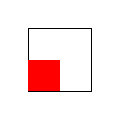
\begin{tikzpicture}[baseline=+2.0ex, scale=0.2]
   \draw         (0,0) rectangle  (4,4);
  \fill[red]    (0,0) rectangle (2,2);
 \end{tikzpicture},  \quad
  
\begin{tikzpicture}[baseline=+2.0ex, scale=0.2]
   \draw         (0,0) rectangle  (4,4);
  \fill[red]    (2,0) rectangle (4,2);
 \end{tikzpicture},   \\
 & 
 \qquad \quad 
\begin{tikzpicture}[baseline=+2.0ex, scale=0.2]
   \draw         (0,0) rectangle  ++ (4,4);
  \fill[red]    (0,0) rectangle  ++ (2,4);
 \end{tikzpicture},  \quad 
 
\begin{tikzpicture}[baseline=+2.0ex, scale=0.2]
  \draw         (0,0) rectangle  ++ (4,4);
  \fill[red]    (2,0) rectangle  ++ (2,4);
  \end{tikzpicture}, \quad
 
\begin{tikzpicture}[baseline=+2.0ex, scale=0.2]
   \draw         (0,0) rectangle  (4,4);
  \fill[red]    (0,2) rectangle   (4,4);
 \end{tikzpicture},  \quad 
 
\begin{tikzpicture}[baseline=+2.0ex, scale=0.2]
  \draw         (0,0) rectangle   (4,4);
  \fill[red]    (0,0) rectangle   (4,2);
  \end{tikzpicture},\\
 & 
 \qquad \quad 
\begin{tikzpicture}[baseline=+2.0ex, scale=0.2]
   \draw         (0,0) rectangle  (4,4);
  \fill[red]    (0,2) rectangle  (2,4);
   \fill[red]    (2,0) rectangle (4,2);
 \end{tikzpicture},  \quad 
 
\begin{tikzpicture}[baseline=+2.0ex, scale=0.2]
   \draw         (0,0) rectangle  (4,4);
  \fill[red]    (2,2) rectangle   (4,4);
   \fill[red]    (0,0) rectangle (2,2);
 \end{tikzpicture},  \quad  
 
\begin{tikzpicture}[baseline=+2.0ex, scale=0.2]
   \draw         (0,0) rectangle  (4,4);
   \fill[red]         (0,0) rectangle  (4,4);
  \fill[white]    (0,2) rectangle  (2,4);
 \end{tikzpicture},  \quad 

\begin{tikzpicture}[baseline=+2.0ex, scale=0.2]
   \draw         (0,0) rectangle  (4,4);
   \fill[red]         (0,0) rectangle  (4,4);
  \fill[white]    (2,0) rectangle (4,2);
 \end{tikzpicture},  \quad 

\begin{tikzpicture}[baseline=+2.0ex, scale=0.2]
   \draw         (0,0) rectangle  (4,4);
   \fill[red]         (0,0) rectangle  (4,4);
  \fill[white]    (0,0) rectangle (2,2);
 \end{tikzpicture},  \quad 

\begin{tikzpicture}[baseline=+2.0ex, scale=0.2]
   \draw         (0,0) rectangle  (4,4);
   \fill[red]         (0,0) rectangle  (4,4);
  \fill[white]      (2,2) rectangle (4,4);
 \end{tikzpicture},  \quad 
 
\begin{tikzpicture}[baseline=+2.0ex, scale=0.2]
   \draw         (0,0) rectangle  (4,4);
  \fill[red]    (0,0) rectangle  (4,4);
 \end{tikzpicture}
 \Bigg\} \\
 \vdots & \qquad \qquad \qquad \vdots 
 \end{align*} 
 	

Then $\set{\F_n}$ is a filtration.
\end{frame}


\begin{frame}{Martingales}
	
\begin{definition}
Let $\set{X_n}$ be a sequence of random variables  and $\set{\F_n}$ be a filtration.    If
%
\begin{enumerate}
\item The sequence $\set{X_n}$ is adapted to the filtration $\set{\F_n}$.
\item Each $X_n$ is integrable.
\item $\E[X_{n+1} \cond \F_n] = X_n \quad \text{for all} \; n.$
\end{enumerate}
%
Then we say that $\set{X_n}$ is a \textbf{martingale} relative to $\set{\F_n}$.  

If, in the last definition, $=$ is replaced by $\leq$ or $\geq$, then $\set{X_n}$ is said to be a \textbf{supermartingale} or \textbf{submartingale}, respectively.
\label{def:martingale_supermartingale_and_submartingale}
\end{definition}

\end{frame}

\begin{frame}{Examples of Martingales}
\begin{enumerate}
	\item Random walks. 
	\item Polya Urn process.
	\item Increasing information process. (See next slides.)
\end{enumerate}
	
\end{frame}

\begin{frame}{Concrete example of increasing information process}

We define a probability space as follows:
%
\begin{align*}
\Omega &= [0,1]^2 \quad \tinytext{(the unit square)} \\
\F &= \B([0,1]^2) \\
P &= \text{Uniform distribution}
\end{align*}
%
To construct a filtration, we begin by constructing a sequence $\set{\Omega_n}$ of increasingly refined partitions of $\Omega$. We set
%
\begin{align*}
\Omega_0 &= \bigg\{ \emptyset, \Omega \bigg\} \\
\Omega_n & \; \text{as the partition of $\Omega$ formed by splitting cells of $\Omega_{n-1}$ in half} \\
& \; \text{ vertically if $n$ odd and horizontally if $n$ even} \\
\end{align*} 	
%
We then define a filtration by setting $\F_n = \sigma(\Omega_n)$, i.e. each $\sigma$-field $\F_n$ consists of the sets that can be formed by taking unions of some subset of the cells in the partition $\Omega_n$.  
\end{frame}


\begin{frame}{Concrete example of increasing information process}
\scriptsize Now let $Y$ be an integrable random variable on $(\Omega, \F, P)$, and define $X_n = \E[Y \cond \F_n]$. For example:
%
\begin{figure}[H]
\centering
\includegraphics[width=.4\textwidth]{images/example_of_increasing_information_process.png}	
\end{figure}
For the first few elements in the sequence ($n=1,\hdots,4$), we show the values of the random variable $X_n \defeq \E[Y \cond \F_n]$ over each element of a partition $\Omega_n$ from which the $\sigma$-field $\F_n$ is generated.
\end{frame}

\begin{frame}

The Figure illustrates the martingale property: $X_n = \E[X_{n+1} \cond \F_n]$.  In particular, we can see that both conditions for conditional expectation  are satisfied:
%
\begin{itemize}
\item \textbf{average matching}: for any set in $\F_n$ (which is a rectangle or union of rectangles in the partition $\Omega_n$), the value of $X_n$ is the arithmetic average of the values of the corresponding subrectangles in $\F_{n+1}$.
\item \textbf{measurability}: inverse images of any realization $X_n = x_n$ or set of realizations $X_n \in  \set{x_n^^1, \hdots x_n^^k}$ exist in $\F_n$.
\end{itemize}

The Figure also illustrates what we mean by an ``increasing information" process:
\begin{itemize}
\item As $n$ increases, $X_n$ gives more information about the values of $Y$ on the square $\Omega$. 
\vskip.02in
{\scriptsize (In particular, $X_n$ gives us the average value of $Y$ over a grid of sub-rectangles that is a refinement of the corresponding grid over which $X_{n-1}$ gave averages.  Every time we split a rectangle in half, the original value $a$ splits into two values $b$ and $c$ such that $a = \frac{b+c}{2}$.  There are of course infinitely many possible choices for $b$ and $c$ given $a$, and we don't know what those values are until we observe the next random variable in the sequence.) }	
\end{itemize}

	
\end{frame}

\begin{frame}{The increasing information process is a martingale}
\begin{proposition}
Let $Y$ be an integrable random variable and $\F_n$ be a filtration on $(\Omega, \F, P)$. 
Define
\[ X_n \defeq \E[Y \cond \F_n]\]
Then $X_n$ is a martingale with respect to $\F_n$.
\end{proposition}

\begin{proof}
The first two conditions of the definition follow immediately.  For the third condition, note that 
\begin{align*}
\E[X_{n+1} \cond \F_n] &= \E \big[ \E[Y \cond \F_{n+1}] \cond \F_n \big] && \tinytext{def. $\set{X_n}$} \\
&= \E[Y \cond \F_n] && \tinytext{``Smaller $\sigma$-field always wins", a.k.a. the tower property} \\
&= X_n && \tinytext{def. $\set{X_n}$}
\end{align*}	
\end{proof}
	
\end{frame}


\end{document}